\section{Numerical Implementation}
\label{sec:numerics}

A KAN-ODE is two numerical objects stacked on top of each other: a
function approximator that evaluates the vector field $\mathbf f_\theta$, and
an explicit integrator that turns that field into a trajectory. Training
differentiates through both. This section gives the exact computation for
each, the cost of one training epoch in terms of them, and the three
structural modifications to the field that later sections use as fixes.

\subsection{Where the implementation comes from}

The paper's own code \cite{koenig2024kanoderepo} is written in Julia and
builds its network from the \texttt{KDense} layer of
\texttt{Kolmogorov\-Arnold.jl} \cite{puri2024kolmogorovarnoldjl}, a KAN
library that evaluates every edge's basis functions as one dense array
operation instead of one spline object per edge. This project ports that
layer to PyTorch rather than using \texttt{pykan} \cite{liu2024kan}, the
reference Python KAN implementation. \texttt{pykan} stores a separate
B-spline object on each edge and periodically refits its grid during
training, which is flexible but slow and makes the basis hard to swap. The
\texttt{KDense} formulation reduces a whole layer to one basis tensor and one
matrix product (Algorithm~\ref{alg:kdense}), so replacing the basis is a
change to a single function, and every basis in this report is evaluated by
exactly the same code path. The integrators, the training loop and every
diagnostic were written for this project and not taken from an ODE library,
so that each solver could be instrumented identically. Two library
components are used only as independent baselines: the continuous-adjoint
gradient in Section~\ref{sec:track-a} comes from \texttt{torchdiffeq}
\cite{torchdiffeq}, and the sparse regression of Section~\ref{sec:track-e}
from \texttt{pysindy} \cite{desilva2020pysindy,kaptanoglu2022pysindy}.

The port matches \texttt{KDense} in every structural detail: a fixed grid of
$G$ evenly spaced centres on $[-1,1]$ with spacing $h=2/(G-1)$, a $\tanh$
normalizer on the basis path, a SiLU residual path applied to the
\emph{unnormalized} input, and Glorot-uniform initialization. It differs in
two numerical details, both recorded in the implementation audit
(Table~\ref{tab:paper-audit}): the Gaussian is
$\exp(-\tfrac12((u-z_g)/h)^2)$, as written in the paper's Equation~5, whereas
the paper's code uses $\exp(-((u-z_g)/h)^2)$, a kernel narrower by a factor
of $\sqrt2$; and the initial weights are not divided by $10^5$ as the
paper's code does.

\subsection{One KAN layer}

Figure~\ref{fig:kan-edge} expands a single edge of the network in
Figure~\ref{fig:kan-ode-architecture}. For an input vector
$\mathbf x\in\mathbb R^{n_{\text{in}}}$, the layer computes
\begin{equation}
y_j \;=\; \sum_{i=1}^{n_{\text{in}}}\phi_{j,i}(x_i)
\;=\; \sum_{i=1}^{n_{\text{in}}}\Big(\,\underbrace{\sum_{g=1}^{G} C_{j,i,g}\,B_g\big(\tanh x_i\big)}_{\text{learned basis expansion}}
\;+\;\underbrace{W_{j,i}\,\mathrm{silu}(x_i)}_{\text{residual path}}\Big),
\qquad j=1,\dots,n_{\text{out}},
\label{eq:kdense}
\end{equation}
with trainable coefficient tensor $C\in\mathbb R^{n_{\text{out}}\times n_{\text{in}}\times G}$
and residual weights $W\in\mathbb R^{n_{\text{out}}\times n_{\text{in}}}$.
Every edge $(i\to j)$ therefore owns its own univariate function
$\phi_{j,i}$, shaped by its own $G$ coefficients. The $\tanh$ is needed
because the basis functions are only defined on the grid's range $[-1,1]$;
it maps any real input into that range. The residual path keeps a direct,
unsquashed route from input to output, which stops the layer from saturating
when an input is large.

\begin{figure}[htbp]
\centering
\begin{tikzpicture}[font=\small,
  io/.style={draw=ink, fill=accentsoft, minimum size=7mm, rounded corners=2pt},
  op/.style={draw=ink!60, fill=codebg, minimum height=7mm, minimum width=13mm, rounded corners=2pt, align=center},
  bas/.style={draw=accent!70, fill=white, minimum width=11mm, minimum height=5.5mm, rounded corners=1pt, font=\scriptsize},
  sumnd/.style={draw=accent, fill=accentsoft, circle, minimum size=7mm, inner sep=0pt, font=\bfseries\color{accent}},
  arr/.style={-{Stealth[length=2mm]}, draw=ink!65, thick}]
  \node[io] (x) at (0,0) {$x_i$};
  \node[op] (nrm) at (1.9,1.0) {$u=\tanh x_i$};
  \node[bas] (b1) at (4.2,2.0) {$B_1(u)$};
  \node[bas] (b2) at (4.2,1.3) {$B_2(u)$};
  \node[font=\scriptsize] at (4.2,0.75) {$\vdots$};
  \node[bas] (bG) at (4.2,0.1) {$B_G(u)$};
  \node[op] (lin) at (6.6,1.05) {$\sum_g C_{j,i,g}\,B_g(u)$};
  \node[op] (silu) at (3.2,-1.2) {$\mathrm{silu}(x_i)$};
  \node[op] (w) at (6.6,-1.2) {$\times\,W_{j,i}$};
  \node[sumnd] (sum) at (8.7,0) {$+$};
  \node[io] (phi) at (10.3,0) {$\phi_{j,i}(x_i)$};
  \draw[arr] (x) |- (nrm);
  \draw[arr] (nrm.east) -- (b1.west);
  \draw[arr] (nrm.east) -- (b2.west);
  \draw[arr] (nrm.east) -- (bG.west);
  \draw[arr] (b1.east) -- (lin.west);
  \draw[arr] (b2.east) -- (lin.west);
  \draw[arr] (bG.east) -- (lin.west);
  \draw[arr] (x) |- (silu);
  \draw[arr] (silu) -- (w);
  \draw[arr] (lin.east) -- (sum);
  \draw[arr] (w.east) -- (sum);
  \draw[arr] (sum) -- (phi);
  \begin{pgfonlayer}{background}
    \node[draw=accent, dashed, thick, rounded corners=4pt, fit=(b1)(bG), inner sep=4pt,
          label={[font=\tiny\sffamily\color{accent}, align=center]above:basis bank:\\the ablated component}] {};
  \end{pgfonlayer}
  \node[font=\tiny\sffamily\color{ink!60}] at (6.6,1.75) {$G$ trainable coefficients};
  \node[font=\tiny\sffamily\color{ink!60}] at (6.6,-1.75) {1 trainable weight};
  \node[font=\tiny\sffamily\color{ink!60}, align=center] at (1.9,1.7) {maps into the\\grid range $[-1,1]$};
\end{tikzpicture}
\caption{One edge $\phi_{j,i}$ of a KAN layer (Equation~\ref{eq:kdense}). The
input is squashed into $[-1,1]$, expanded in $G$ fixed basis functions, and
recombined with $G$ learned coefficients; a separate residual path adds a
learned multiple of $\mathrm{silu}(x_i)$. The basis ablation of
Section~\ref{sec:phase2} replaces only the dashed box. In the original KAN
paper that box holds cubic B-splines; the base paper replaces them with
Gaussian RBFs.}
\label{fig:kan-edge}
\end{figure}

Summing Equation~\ref{eq:kdense} over edges collapses the whole layer into
two matrix products. Stacking the basis values of all inputs into one vector
$\boldsymbol\beta(\mathbf x)\in\mathbb R^{n_{\text{in}}G}$ and reshaping $C$
into an $n_{\text{out}}\times n_{\text{in}}G$ matrix gives
\begin{equation}
\mathbf y \;=\; C\,\boldsymbol\beta(\mathbf x) \;+\; W\,\mathrm{silu}(\mathbf x),
\label{eq:kdense-matrix}
\end{equation}
which is what Algorithm~\ref{alg:kdense} evaluates, for a whole batch of
states at once.

\begin{algorithm}[htbp]
\caption{Forward pass of one KAN layer (tensor shapes in brackets; $b$ is the batch size).}
\label{alg:kdense}
\begin{algorithmic}[1]
\Require states $X\,[b\times n_{\text{in}}]$; grid $\mathbf z\,[G]$, spacing $h$; coefficients $C\,[n_{\text{out}}\times n_{\text{in}}G]$; residual weights $W\,[n_{\text{out}}\times n_{\text{in}}]$
\Ensure layer output $Y\,[b\times n_{\text{out}}]$
\State $U \gets \tanh(X)$ \Comment{$[b\times n_{\text{in}}]$, now inside $[-1,1]$}
\State $\mathcal B[\,\cdot,i,g] \gets B_g(U[\,\cdot,i];\,\mathbf z,h)$ for all $i,g$ \Comment{one broadcast call, $[b\times n_{\text{in}}\times G]$}
\State $\mathcal B \gets \mathrm{reshape}(\mathcal B,\ b\times n_{\text{in}}G)$
\State $Y \gets \mathcal B\,C^{\top}$ \Comment{one matrix product for every edge's expansion}
\State $Y \gets Y + \mathrm{silu}(X)\,W^{\top}$ \Comment{residual path on the unnormalized input}
\State \Return $Y$
\end{algorithmic}
\end{algorithm}

The full vector field is two such layers, $\mathbf f_\theta=\mathrm{KDense}_2\circ\mathrm{KDense}_1$.
Because line~2 is the only place the basis appears, all seven bases compared
in this report (Figure~\ref{fig:basis-shapes}) share lines 1 and 3--6 exactly.

\begin{figure}[htbp]
\centering
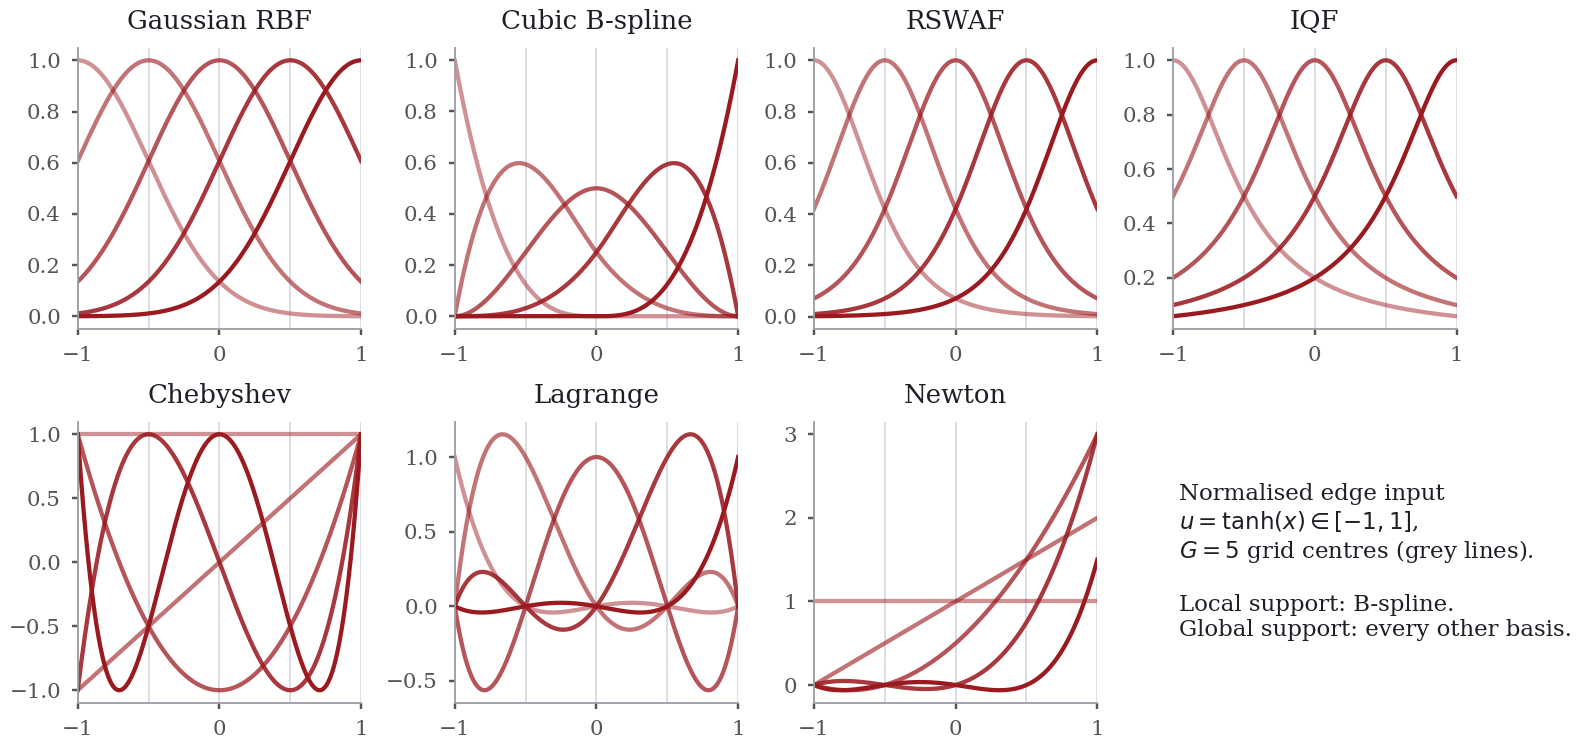
\includegraphics[width=\linewidth]{figures/methods/basis_functions.png}
\caption{The seven basis families $B_g(u)$ available to line~2 of
Algorithm~\ref{alg:kdense}, evaluated by this project's own implementation
at $G=5$. Only the cubic B-spline has compact support: each of its functions
is exactly zero outside a few neighbouring grid cells. Every other basis is
nonzero almost everywhere, so each coefficient affects the edge function over
the whole input range. Equations~\ref{eq:basis-rbf-spline}--\ref{eq:basis-rational}
give their formulas.}
\label{fig:basis-shapes}
\end{figure}

\paragraph{Cost of one field evaluation.} Lines 4--5 of
Algorithm~\ref{alg:kdense} perform $n_{\text{out}}n_{\text{in}}(G+1)$
multiply-adds per state, which is exactly the layer's parameter count
(Equation~\ref{eq:param-count}), so the $[2,10,2]$, $G=5$ network costs 240
multiply-adds per evaluation of $\mathbf f_\theta$. Line~2 costs
$O(n_{\text{in}}G)$ elementwise operations for the RBF, RSWAF and IQF kernels,
which are single closed-form expressions. The cubic B-spline uses a clamped
(open-uniform) knot vector: each boundary knot is repeated $k+1=4$ times,
with $G-k-1$ evenly spaced interior knots, so its $G$ basis functions sum to
exactly one everywhere on $[-1,1]$, including at the edges. It then runs the
Cox--de Boor recursion, which rebuilds the basis over four degree levels with
two divisions per knot interval at each level. Since the matrix product is
identical for every basis, this extra basis work is the most likely reason
the B-spline run takes $3.9\times$ the RBF run's wall-clock time at the same
parameter count (Table~\ref{tab:basis-ablation}). The time was measured; the
breakdown of where it goes was not profiled.

\subsection{The integrator}

Every solver in this report is an explicit Runge-Kutta method. An $s$-stage
method advances the state by a step $h$ as
\begin{equation}
\mathbf k_i=\mathbf f_\theta\Big(\mathbf u_n+h\sum_{j=1}^{i-1}a_{ij}\,\mathbf k_j\Big),\quad i=1,\dots,s,
\qquad
\mathbf u_{n+1}=\mathbf u_n+h\sum_{i=1}^{s}b_i\,\mathbf k_i,
\label{eq:rk-general}
\end{equation}
where the coefficients $(a_{ij},b_i,c_i)$ form the method's Butcher tableau.
Euler, Midpoint, Heun and RK4 (Equations~\ref{eq:euler}--\ref{eq:rk4}) are
special cases with $s=1,2,2,4$; DOPRI5 \cite{dormand1980dopri} and Tsit5
\cite{tsitouras2011tsit5} use $s=7$ tableaus, listed in full in
Appendix~\ref{app:butcher}. Both are ``first same as last'' methods whose
seventh stage has zero solution weight ($b_7=0$). It exists only to feed the
embedded error estimate used for adaptive step control. Since this project
integrates with a fixed step, that stage is skipped, and both methods cost
six field evaluations per step.

\paragraph{Fixed steps and substeps.} The base paper integrates with
\emph{adaptive} Tsit5, which chooses its own step from an error estimate.
This project uses a \emph{fixed} step instead, so that the number of
function evaluations, and hence the backpropagation graph, is identical
every epoch and can be compared across solvers. Between two consecutive
observation times the solver takes $m$ equal substeps
(Algorithm~\ref{alg:odeint}); every run in this report uses $m=2$, so the
integration step is $h=\Delta t/2$ (0.05 for Lotka-Volterra, not the data
spacing of 0.1).

\begin{algorithm}[htbp]
\caption{Fixed-step trajectory integration with substeps.}
\label{alg:odeint}
\begin{algorithmic}[1]
\Require field $\mathbf f_\theta$; initial state $\mathbf u_0$; observation times $t_0<\dots<t_N$; one-step map $\Phi_h$ (Eq.~\ref{eq:rk-general}); substeps $m$
\Ensure predicted states $\hat{\mathbf u}(t_0),\dots,\hat{\mathbf u}(t_N)$
\State $\hat{\mathbf u}(t_0)\gets\mathbf u_0$;\ \ $\mathbf u\gets\mathbf u_0$
\For{$n=0,\dots,N-1$}
  \State $h\gets (t_{n+1}-t_n)/m$
  \For{$r=0,\dots,m-1$}
    \State $\mathbf u\gets\Phi_h(\mathbf f_\theta,\ t_n+r h,\ \mathbf u)$ \Comment{$s$ evaluations of $\mathbf f_\theta$}
  \EndFor
  \State $\hat{\mathbf u}(t_{n+1})\gets\mathbf u$
\EndFor
\State \Return $\hat{\mathbf u}(t_0),\dots,\hat{\mathbf u}(t_N)$
\end{algorithmic}
\end{algorithm}

A training epoch therefore evaluates the field
\begin{equation}
\mathrm{NFE}_{\text{epoch}}=(N_{\text{train}}-1)\,m\,s
\label{eq:nfe}
\end{equation}
times. For Lotka-Volterra, $N_{\text{train}}=36$ and $m=2$, giving 70 for
Euler, 140 for the second-order methods, 280 for RK4 and 420 for DOPRI5 and
Tsit5, which are the values in Table~\ref{tab:solver-ablation}. Because
backpropagation keeps every intermediate stage (Section~\ref{sec:track-a}),
$\mathrm{NFE}_{\text{epoch}}$ also sets the memory and time of the backward
pass.

\paragraph{Accuracy.} A method of order $p$ commits a local truncation error
of $O(h^{p+1})$ per step, which accumulates to a global error of $O(h^{p})$
over a fixed horizon \cite{hairer1993solving}:
\begin{equation}
\big\lVert \mathbf u_n-\mathbf u(t_n)\big\rVert \le K\,h^{p}\qquad\text{for } t_n\le T,
\label{eq:global-error}
\end{equation}
with $K$ depending on $T$ and on the smoothness of the field. Halving $h$
should therefore reduce the error by $2^{p}$: by 2 for Euler, 4 for Midpoint
and Heun, 16 for RK4, and 32 for the fifth-order methods. The solver test
suite (Section~\ref{sec:verification}) checks exactly this on ODEs with known
solutions.

\paragraph{Stability.} Applied to the linear test equation
$\dot u=\lambda u$, an explicit method reduces to $u_{n+1}=R(z)\,u_n$ with
$z=h\lambda$ and a polynomial stability function
\begin{equation}
R_{\text{Euler}}(z)=1+z,\qquad
R_{\text{RK2}}(z)=1+z+\tfrac{z^2}{2},\qquad
R_{\text{RK4}}(z)=\sum_{k=0}^{4}\frac{z^k}{k!},
\label{eq:stability-function}
\end{equation}
and the numerical solution decays, as the true solution does for
$\operatorname{Re}\lambda<0$, only while $|R(z)|\le1$
\cite{hairer1996solving}. On the negative real axis this holds for
$h|\lambda|\le2$ (Euler and both second-order methods) and
$h|\lambda|\lesssim2.79$ (RK4). A polynomial $R$ always grows without bound
for large $|z|$, so every explicit method has a bounded stability region;
this is the classical reason explicit solvers fail on stiff problems, and it
is the prediction the damping study (Section~\ref{sec:track-d}) tests
against the trained models.

\subsection{Differentiating through the solver}

The loss (Equation~\ref{eq:train-loss}) depends on $\theta$ only through the
integrated trajectory. This project computes its gradient by
\emph{direct automatic differentiation}: every operation of
Algorithms~\ref{alg:kdense}--\ref{alg:odeint} is recorded, and the reverse
pass applies the chain rule back through all $\mathrm{NFE}_{\text{epoch}}$
field evaluations. The result is the exact gradient of the discrete
computation, at a memory cost linear in the number of steps. The base paper
instead uses the continuous adjoint method, which solves a second ODE
backward in time; Section~\ref{sec:track-a} derives it and measures which of
the two is cheaper at this project's scale.

\subsection{Structural modifications of the field}

Three optional wrappers change \emph{what} is integrated without changing the
network itself. Each is used as a fix in Section~\ref{sec:phase2} and tested
for transfer in Section~\ref{sec:track-e}.

\paragraph{Time rescaling.} With a scale factor $s$, the model is integrated
in rescaled time $\tau=t/s$, so the network learns
$\mathbf g_\theta=s\,\mathbf f$ instead of $\mathbf f$:
\begin{equation}
\frac{\dd\mathbf u}{\dd\tau}=\mathbf g_\theta(\mathbf u),\qquad \hat{\mathbf u}(t)=\hat{\mathbf u}(\tau=t/s).
\label{eq:time-scale}
\end{equation}
This is a change of units only. It lets a system whose true rates are small
(SIR's rates are $\sim10^{-2}$ per day) be learned by a network whose
initial output is $\sim10^{-1}$, without changing the dynamics being fit.

\paragraph{Zero-sum projection.} For a system whose state components must sum
to a constant, the field is projected onto the zero-sum subspace,
\begin{equation}
\mathbf f_{\text{proj}}(\mathbf u)=\mathbf f_\theta(\mathbf u)-\frac1d\sum_{k=1}^{d}f_{\theta,k}(\mathbf u)\,\mathbf 1,
\qquad\text{so}\qquad \frac{\dd}{\dd t}\sum_k u_k=\sum_k f_{\text{proj},k}=0 .
\label{eq:projection}
\end{equation}
The invariant then holds for every state and every horizon, up to rounding
error, rather than only where a penalty term was fitted. Every Runge-Kutta
step is a linear combination of field values, so a zero-sum field gives a
zero-sum update at any order and any step size.

\paragraph{Vanishing-field gate.} For compartmental epidemic models every
transition is proportional to the infected fraction, so $I=0$ is a line of
equilibria: a population with no infection stays that way. The gate builds
this in by multiplying the field by one state component $u_d$,
\begin{equation}
\mathbf f_{\text{gate}}(\mathbf u)=u_d\,\mathbf f_\theta(\mathbf u),
\label{eq:vanishing-gate}
\end{equation}
so that $\mathbf f_{\text{gate}}=\mathbf 0$ whenever $u_d=0$. For SIR
($d=I$) the true field is $I$ times a cofactor that is affine in $S$, which
leaves the network a much simpler function to learn. Unlike the other two
wrappers, this one makes a physical assumption about the system.

\paragraph{The training loop.} Algorithm~\ref{alg:train} assembles the pieces.
Its two safety mechanisms were added one after the other, in response to the
cross-domain failures of Section~\ref{sec:phase2}. Gradient clipping, which
bounds the size of one optimizer step, was added after the first, unclipped
pendulum and SIR runs showed gradient-norm explosions. The non-finite guard,
which skips any step whose gradient has overflowed, was added after the
clipped SIR run of Section~\ref{sec:phase2} still ended in NaN. Clipping
alone cannot handle an overflow: rescaling an infinite gradient produces
$\infty\times0=$ NaN, which corrupts every parameter. The 10{,}000-epoch
Lotka-Volterra benchmarks of Section~\ref{sec:phase2} predate both
mechanisms and ran unclipped.

\begin{algorithm}[htbp]
\caption{Training loop used for every run.}
\label{alg:train}
\begin{algorithmic}[1]
\Require training data $\{(t_n,\mathbf u_n)\}_{n<N_{\text{train}}}$; model $\mathbf f_\theta$ (optionally wrapped by Eqs.~\ref{eq:time-scale}--\ref{eq:vanishing-gate}); learning rate $\eta$; clip threshold $c$; epochs $E$
\Ensure checkpoint $\theta^{\star}$ with the lowest training loss
\State $\mathcal L^{\star}\gets\infty$;\ \ initialize $\theta$ (Glorot uniform), Adam state
\For{$e=1,\dots,E$}
  \State $\hat{\mathbf u}\gets$ Algorithm~\ref{alg:odeint}$(\mathbf f_\theta,\mathbf u_0,t_{0:N_{\text{train}}-1})$
  \State $\mathcal L\gets$ Equation~\ref{eq:train-loss};\ \ $\mathbf g\gets\nabla_\theta\mathcal L$ \Comment{direct autograd through the solver}
  \If{$\mathcal L<\mathcal L^{\star}$} \State $\mathcal L^{\star}\gets\mathcal L$;\ \ $\theta^{\star}\gets\mathrm{copy}(\theta)$ \Comment{weights that produced $\mathcal L$}
  \EndIf
  \If{$\lVert\mathbf g\rVert$ and $\mathcal L$ are finite}
    \State \textbf{if} clipping is enabled \textbf{then} $\mathbf g\gets\mathbf g\cdot\min(1,\,c/\lVert\mathbf g\rVert)$
    \State $\theta\gets\mathrm{Adam}(\theta,\mathbf g,\eta)$
  \Else
    \State skip the update; abort if 100 consecutive steps are non-finite
  \EndIf
  \State every 10 epochs: record loss on the full horizon \Comment{monitoring only, never used for selection}
\EndFor
\State \Return $\theta^{\star}$
\end{algorithmic}
\end{algorithm}

\FloatBarrier
